
\subsubsection{01.10.14}

\begin{enumerate}
	\item The time of beginning and ending of the congregation:
	18:00 - 21:30
	\item Purposes of the congregation:
	\begin{enumerate}
		\item Chose and create wheelbase of our robot.
		
		\item Write simple programme to control motions of the robot by means of joystick.
		
	\end{enumerate}
	
	\item Results:
	\begin{enumerate}
		\item Weelbase was created:
		\begin{enumerate}
			\item Preference was given to the omni- wheels with a roller disposed at an angle of 45 degrees to the direction of rotation. However, we hadn't got such weels. That is why we used usual weels instead of omni-weels.
			
			\item We try to dislocate heaviest details as close to the earth, as possible. So,  in the lower part of the robot was located Battery, NXT microcontroller and drivers of the motors and servo-motors. 
			
			\item Wires could accidentally climb out and cling to the other robots or to the own moving parts. So we decided protect the wires from the bottom.
			
			\begin{figure}[H]
				\begin{minipage}[h]{0.2\linewidth}
					\center  
				\end{minipage}
				\begin{minipage}[h]{0.6\linewidth}
					\center{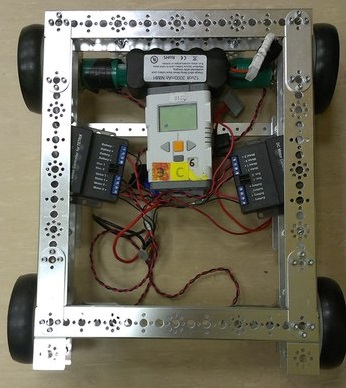
\includegraphics[scale=0.5]{days/01.10.14/images/01}}
					\caption{The ideas of fixing of the movable basket: 1)Capture, that look likes as russian letter "П" 2)Capture with hooks}
				\end{minipage}
			\end{figure}
			
		\end{enumerate}
		
		\item There was idea to create lift like as convair. Such system could lead to the capture of balls fixed on the body of the robot, and raise only balls. So, there are some ideas:
		\begin{enumerate}
			\item Convair with baskets, that are located at equal distances
			\item Sliding hollow cylinder, in which axes, that lift balls, can move.			
			\begin{figure}[H]
				\begin{minipage}[h]{0.2\linewidth}
					\center  
				\end{minipage}
				\begin{minipage}[h]{0.6\linewidth}
					\center{
\includegraphics[scale=0.25]{days/01.10.14/images/02}}
					\caption{Ideas for ball's lift: 1)Convair with baskets 2)Construction with sliding hollow cylinder
				\end{minipage}
			\end{figure}
			
		\end{enumerate}
		
	\end{enumerate}
	
	\item Results: 
	\begin{enumerate}
		\item Wheelbase of the robot was been assembled.
		
		\item Programm wasn't been realised.
		
	\end{enumerate}
	
	\item Tasks for the next congregations:
	\begin{enumerate}
		\item Realised robot's programm.
		
		\item Install underbody protection.
		
	\end{enumerate}     
\end{enumerate}
\fillpage

